\chapter{Descripción del diseño de la base de datos}\label{chapter:database}

El diseño de base de datos es un proceso fundamental a la hora 
de modelar el conjunto de datos y las operaciones que se deseen
realizar sobre ellos. Un correcto diseño de la base de datos
es esencial para garantizar la consistencia de la información,
eliminar datos redundantes, ejecutar consultas de manera 
eficiente y mejorar el rendimiento de la base de datos \cite{db_book_cap2}. 

En este capítulo se presenta el diseño de la base de datos que se 
obtuvo siguiendo el enfoque relacional.
En las secciones \ref{database:asignación-docencia} y
\ref{database:planificación-tesis} se describen las modelaciones que se obtuvieron 
para los procesos de asignación de docencia y planificación de las tesis, respectivamente.






\section{Modelación de la asignación de docencia}\label{database:asignación-docencia}
% Para la modelación del proceso de asignación de docencia, 
% se definieron las entidades fundamentales, así como las interrelaciones que se establecen entre ellas, 
% a partir del modelo entidad-relación extendido. 
% En la figura \ref{} se muestra un
% Como resultado se obtuvo 
% el siguiente esquema
Para informatizar la asignación de docencia, fue 
necesario almacenar toda la información que interviene en este proceso.
Para ello, se modelaron las entidades fundamentales, así como las interrelaciones
que se establecen entre ellas. En la figura \ref{merxx-docencia} se muestra el esquema que se obtuvo a partir 
del modelo entidad-relación.

% Se modelaron las entidades fundamentales
% que intervienen en el proceso de la asignación de docencia, 
% así como las interrelaciones que se establecen entre ellas.
% En la figura \ref{merxx-docencia} se muestra el esquema que se obtuvo a partir 
% del modelo entidad-relación extendido.

\begin{figure}[H]
    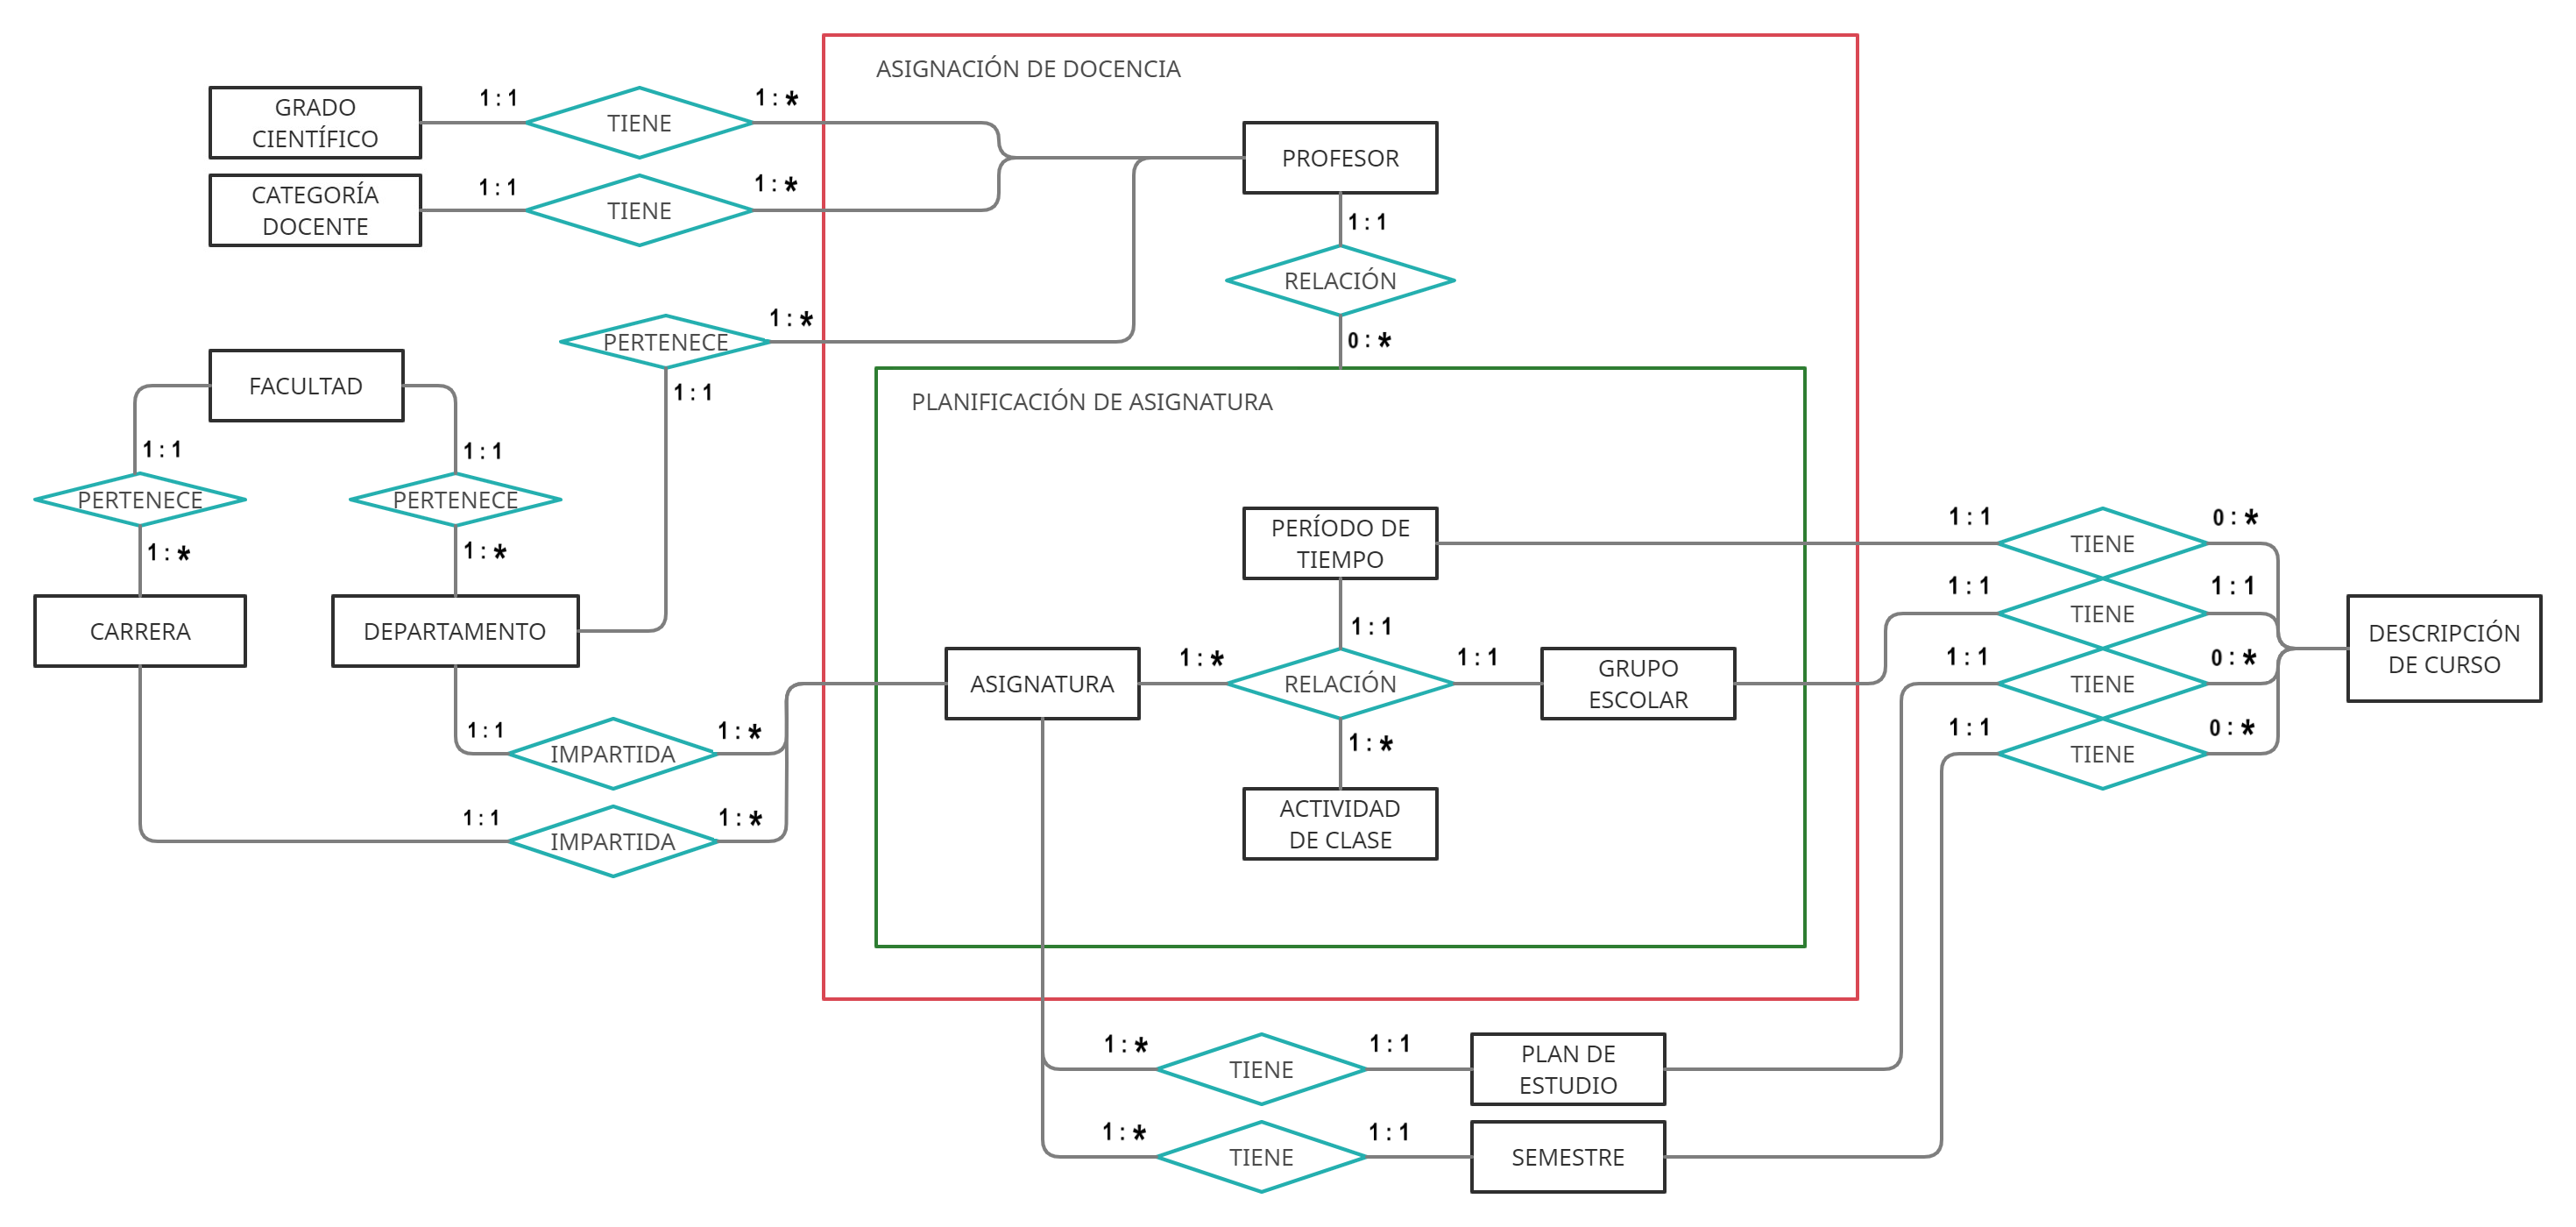
\includegraphics[scale=0.25]{Graphics/Database/MERXX-TA-FINAL.png}
    \caption{MER para la asignación de docencia}
    \label{merxx-docencia}
    
\end{figure}


Con el objetivo de simplificar la representación del modelo entidad-relación
no se agregaron en la imagen \ref{merxx-docencia} los atributos correspondientes a cada entidad,
a continuación se describen los detalles de cada una.


\subparagraph{FACULTAD:}
Representa las facultades de la Universidad de La Habana.
El nombre de la facultad se modela como un atributo, mientras que 
las carreras que se estudian en la facultad y los departamentos que pertenecen 
a ella, se modelan como relaciones con las entidades CARRERA y DEPARTAMENTO, respectivamente.
Una facultad tiene uno o muchos departamentos, y en 
una facultad se pueden estudiar una o más carreras.

\subparagraph{CARRERA:}
Representa las carreras que se estudian en la Universidad de La Habana.
El nombre de la carrera se modela como un atributo, mientras que la facultad a la que pertenece la carrera y
las asignaturas que se imparten en ella, se modelan como relaciones con las entidades FACULTAD y
ASIGNATURA, respectivamente. 
Una carrera pertenece a una única facultad y en una carrera se imparten una o muchas asignaturas.

\subparagraph{DEPARTAMENTO:}
Representa los departamentos de una facultad de la Universidad de La Habana.
El nombre del departamento se modela como un atributo, mientras que los profesores que 
pertenecen a un departamento, las asignaturas que son atendidas por el departamento y la 
facultad a la que pertenece el departamento, se modelan como relaciones con las entidades 
PROFESOR, FACULTAD y ASIGNATURA, respectivamente. Un departamento pertenece a una única facultad,
atiende una o muchas asignaturas y a un departamento pertenecen uno o muchos 
profesores.

\subparagraph{PROFESOR:}
Agrupa los datos asociados a los profesores.
Los campos nombre y apellidos se modelan como atributos,  
mientras que la categoría docente, el grado 
científico de un profesor y el departamento al que pertenece, se modelan como 
relaciones con las entidades CATEGORÍA DOCENTE, GRADO CIENTÍFICO y 
DEPARTAMENTO, respectivamente. Un profesor pertenece a un único departamento y puede tener solo 
un grado científico y una categoría docente. 


\subparagraph{CATEGORÍA DOCENTE:}
Representa la categoría docente que tienen los profesores.
El nombre de la categoría docente se modela como un atributo. 
Pueden existir uno o muchos profesores con una misma categoría docente.

\subparagraph{GRADO CIENTÍFICO:}
Representa el grado científico que tienen los profesores.
El nombre del grado científico se modela como un atributo.
Pueden existir uno o muchos profesores con un mismo grado científico.





\subparagraph{ASIGNATURA:}
Agrupa los datos asociados a las asignaturas.
Los campos nombre de la asignatura y cantidad de horas 
totales a impartir, se modelan como atributos, mientras que
el plan de estudio asociado a la asignatura, el semestre en el que se 
imparte, el departamento responsable de la asignatura y la carrera a la 
que pertenece, se modelan como relaciones con las entidades
PLAN DE ESTUDIO, SEMESTRE, DEPARTAMENTO y CARRERA respectivamente. Una asignatura 
se atiende por un único departamento, pertenece a una única carrera, se imparte en un 
único semestre y tiene un único plan de estudio. Las asignaturas que se imparten de forma 
anual se deben representar como dos asignaturas independientes.

\subparagraph{PLAN DE ESTUDIO:}
Representa el plan de estudio por el que se rige una asignatura.
El nombre del plan de estudio se modela como un atributo.
Pueden existir una o muchas asignaturas con el mismo plan de estudio.



\subparagraph{SEMESTRE:}
Representa los semestres asociados a una carrera. 
El nombre del semestre se modela como un atributo.
Pueden existir una o muchas asignaturas que se impartan en 
el mismo semestre. 

\subparagraph{PERÍODO DE TIEMPO:}
Representa los períodos de tiempo en los que se imparten clases, por ejemplo, enero--julio.
El nombre del período de tiempo se modela como un atributo.


\subparagraph{CURSO ESCOLAR:}
Representa los curso escolares, por ejemplo: 2020-2021.
El nombre del curso de escolar se modela como un atributo. Además 
cuenta con un campo booleano que indica si el curso es el vigente.

\subparagraph{AÑO ESCOLAR:}
Representa los años académicos asociados a una carrera, como por ejemplo:
Matemática primer año (M1) o Computación tercer año (C3).
El nombre del año escolar se modela como un atributo.

\subparagraph{ACTIVIDAD DE CLASE:}
Representa los tipos de actividades que se imparten en una asignatura, 
tales como: conferencias, clases prácticas, seminarios, laboratorios, otros. 


\subparagraph{CARGA DE ASIGNATURA:}
Se crea con el objetivo de modelar la separación de una asignatura
según las actividades de clases a impartir durante un período de tiempo, de un curso escolar y para
un año escolar específico. Está compuesta por la agregación de las entidades ASIGNATURA, CURSO ESCOLAR, ACTIVIDAD DE CLASE, AÑO  
ESCOLAR Y PERÍODO DE TIEMPO.
Se agregan los atributos cantidad de horas a impartir y 
la cantidad de grupos totales.
Por ejemplo, para la asignatura Optimización Matemática I, que se imparte 
en el tercer año de la carrera de Matemática, con un total de 64 horas clase, 
se deben crear dos instancia de CARGA DE ASIGNATURA, una con 32 horas 
de conferencias y otra con 32 horas de clases prácticas, para que posteriormente
se puedan asignar los profesores que se ocuparán de impartir estas planificaciones. 



% Entidad creada con el objetivo de separar las distintas actividades 
% que se imparten en una asignatura ( conferencia, clases 
% prácticas, seminarios, laboratorios, otras )  para
% realizar la asignación de docencia. Cuenta con una ASIGNATURA,
% en un PERÍODO DE TIEMPO, con el tipo de ACTIVIDAD DE CLASE y 
% el GRUPO ESCOLAR correspondiente. Por ejemplo, una planificación de
% asignatura pudiera ser (Poner ejemplo real). 
% se hace necesaria 
% la separación de una ASIGNATURA en más de una instancia para representar 
% el tipo de actividad de clase ( conferencia, clases 
% prácticas, seminarios, laboratorios, otras ), que va a recibir un 
% grupo escolar, en un período de tiempo.



\subparagraph{ASIGNACIÓN DE DOCENCIA:}
Representa las asignaciones de la docencia. Una asignación está compuesta
por un PROFESOR y una CARGA DE ASIGNATURA. Además, tiene  
los atributos grupo y porciento. El atributo grupo indica el grupo específico que 
se le asigna al profesor. Por ejemplo, si existen tres grupos de clases prácticas, 
indica cuál de ellos atiende el profesor.
El atributo porciento indica el porcentaje del total de horas a impartir por el profesor 
asignado. Por ejemplo, existen asignaturas en las que el total 
de horas de una actividad de clase, para un mismo grupo, se distribuye entre varios profesores, como es el caso de las
conferencias de la asignatura Modelos de Optimización I (ver tabla \ref{tabla-carga-asignatura-cap2}), que tiene un total
de 32 horas a impartir, que se distribuyen entre la profesora Aymée Marrero 
y el profesor Fernando Rodríguez, 16 horas cada uno. Para modelar este tipo de escenario
se deben crear dos ASIGNACIÓN DE DOCENCIA para la CARGA DE ASIGNATURA correspondiente a las 
conferencias de la asignatura Modelos de Optimización I, y asignar a los profesores 
Aymée Marrero y Fernando Rodriguez con el 50 porciento de las horas cada uno.  
Un profesor puede tener asignada cero o muchas cargas de asignaturas y una carga de 
asignatura puede estar asignada a uno o muchos profesores.

% Representa las asignaciones de profesores a planificaciones de asignaturas.
% Además se agrega un atributo porciento que indica el porcentaje del total de horas 
% a impartir, que asume el profesor asignado. 
% [Hay que añadir el año escolar o la tabla de carmen]

\subparagraph{DETALLES DE AÑO:}
El objetivo de esta entidad es representar el plan de estudio 
por el que se rige un año escolar y el semestre de la carrera en el que 
se encuentra. Está 
compuesta por la agregación de las entidades AÑO ESCOLAR, PLAN DE ESTUDIO y 
SEMESTRE. Por ejemplo, el 
año escolar C4 (cuarto año de Computación), se rige por el plan E y se encuentra en el primer semestre de la carrera.
A partir de los planes de estudio y los semestres en los que se encuentren los años escolares, 
se puede determinar las asignaturas que se deben impartir en un período de tiempo. Por tanto, antes 
de realizar el proceso de asignación de docencia se debe verificar que los datos 
de los años escolares estén actualizados.


% Representa el grupo escolar vigente en el curso actual. Está 
% compuesta por la agregación de las entidades GRUPO ESCOLAR,
% PERÍODO DE TIEMPO, PLAN DE ESTUDIO y SEMESTRE.  
% Por ejemplo, una DESCRIPCIÓN DE CURSO puede ser 
% que el grupo escolar C4 (Computación de cuarto año), con plan de
% estudio E, se encuentra en el semestre 8,  en el período de tiempo septiembre-diciembre.
    



    

\section{Modelación de los tribunales de tesis}\label{database:planificación-tesis}
Para informatizar la planificación de las tesis, fue 
necesario almacenar toda la información que interviene en este proceso.
Para ello, se modelaron las entidades fundamentales, así como las interrelaciones
que se establecen entre ellas. En la figura \ref{merxx-thesis} se muestra el esquema que se obtuvo a partir 
del modelo entidad-relación.


% Se modelaron las entidades fundamentales 
% que intervienen en el proceso de planificación de las tesis, así como 
% las interrelaciones que se establecen entre ellas. En la figura 
% \ref{merxx-thesis} se muestra el esquema que se obtuvo a partir del 
% modelo entidad-relación extendido.


\begin{figure}[H]
    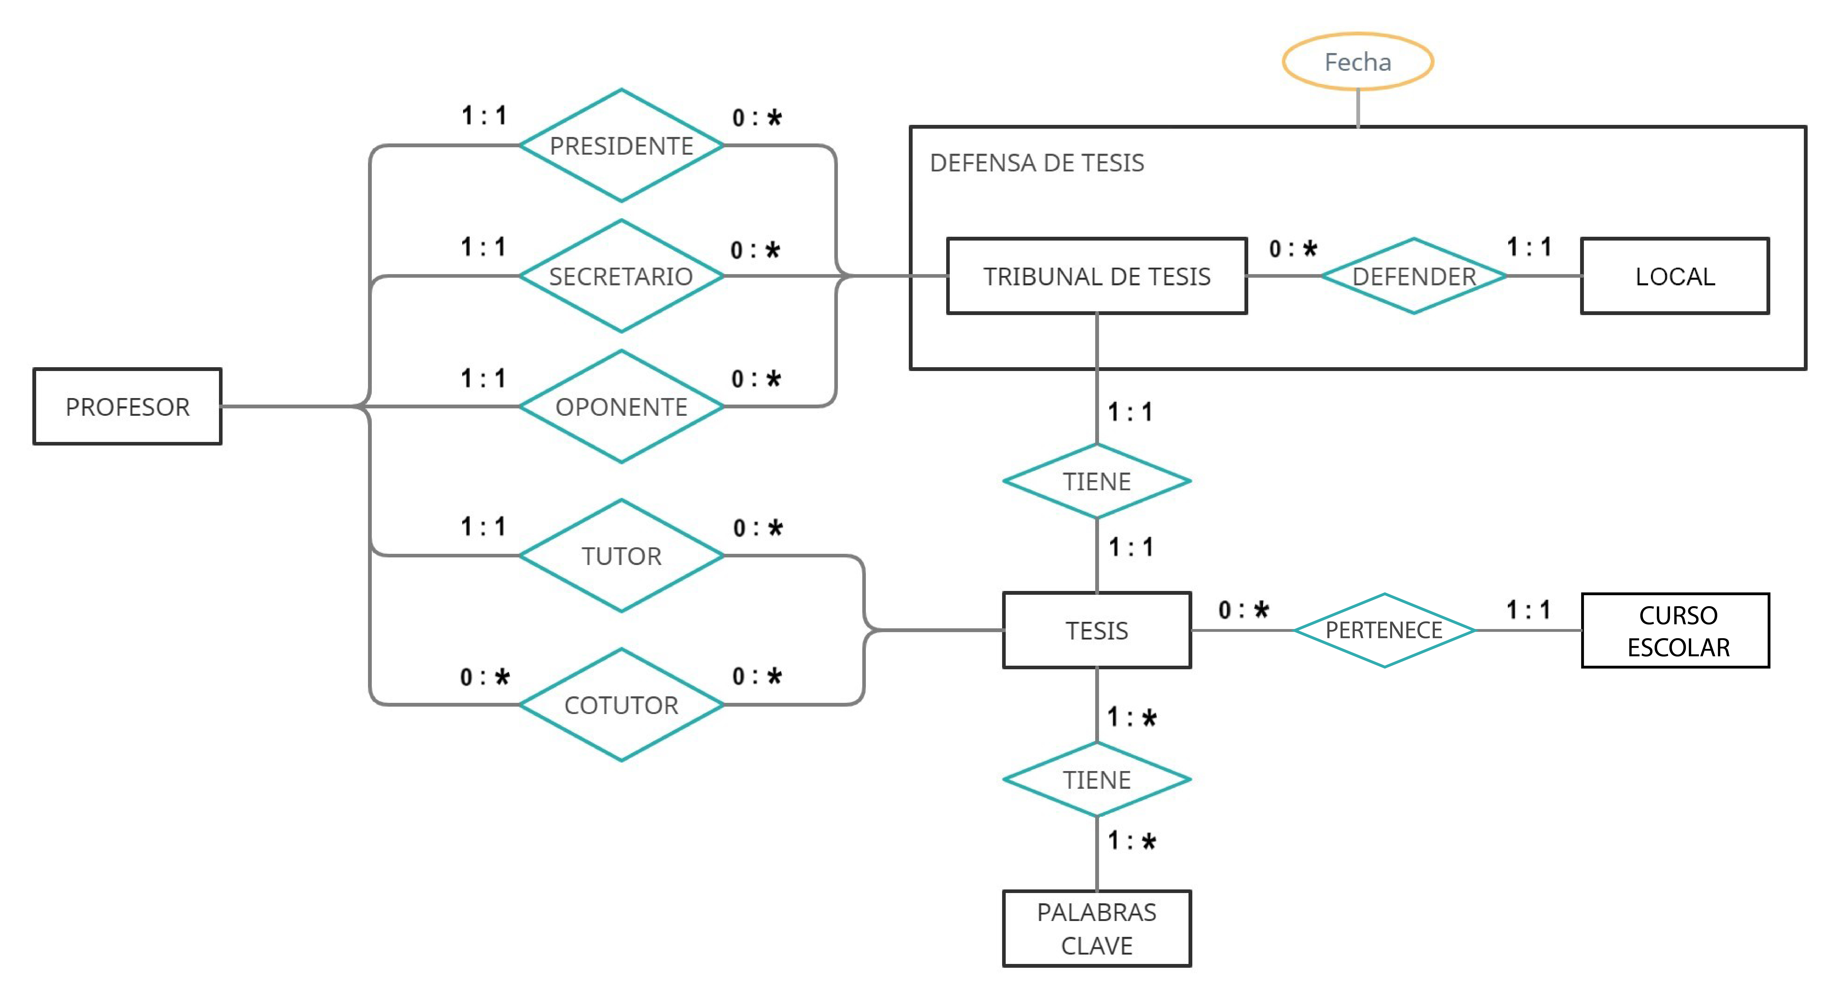
\includegraphics[scale=0.31]{Graphics/Database/MERXX-TC-FINAL.png}
    \caption{MER para la planificación de las tesis}
    \label{merxx-thesis}
\end{figure}


Con el objetivo de simplificar la representación del modelo entidad-relación
no se agregaron en la figura \ref{merxx-thesis} los atributos correspondientes a cada entidad,
a continuación se describen los detalles de cada una.

\subparagraph{TESIS:}
Agrupa los datos asociados a una tesis.
El título de la tesis y el autor se modelan como atributos, mientras que
el tutor, los cotutores, curso escolar y las palabras clave se modelan como relaciones con 
las entidades PROFESOR (tutor y cotutores), CURSO ESCOLAR y PALABRAS CLAVE.
Una tesis tiene un único tutor, puede tener cero o muchos cotutores, pertenece a 
un único curso escolar y tiene una o muchas palabras clave. 

\subparagraph{PALABRAS CLAVE:}
Representa las palabras clave que describen el contenido de una tesis.
El nombre o texto de las palabras clave se modela como un atributo. Una 
palabra clave puede aparecer en una o muchas tesis. 


\subparagraph{TRIBUNAL DE TESIS:}
Representa el tribunal de la defensa de una tesis.
Se compone por los miembros del tribunal: presidente, secretario y oponente, 
y la tesis.
Estos campos se modelan como relaciones con las entidades PROFESOR y TESIS, respectivamente.
Un tribunal de tesis tiene una única tesis, un único presidente, un único secretario y 
un único oponente.


\subparagraph{DEFENSA DE TESIS:}
Representa el acto de defensa de la tesis. 
Se compone por un tribunal de tesis, un local y una 
fecha. La fecha se modela como un atributo, mientras que 
el tribunal y el local se modelan como relaciones con las entidades TRIBUNAL DE 
TESIS y LOCAL, respectivamente. Una defensa de tesis tiene un único tribunal de tesis,
una única fecha y un único local.



\subparagraph{LOCAL:}
Representa el local donde se lleva a cabo la defensa de las tesis.
El nombre del local se modela como un atributo. 
En un local se puede realizar la defensa de cero o muchas tesis.


\subparagraph{PROFESOR:}
Se utiliza la misma entidad creada en el proceso de asignación de docencia.
Un profesor puede tener el rol de presidente, secretario u oponente en cero o 
muchos tribunales de tesis. Un profesor puede ser 
tutor o cotutor de cero o muchas tesis. \\


% DESPUES DE LA MODELACION DE CADA PROCESO CREO Q DEBO HABLAR UN 
% POCO DEL PROCESO DE NORMALIZACION PARA ESOS ESQUEMAS, Y REVISAR SI 
% ESTAN EN 3FN... 

% NO SE QUE MAS MENCIONAR EN ESTE CAPITULO.

En el próximo capítulo se presenta el sistema que se implementó en el 
trabajo para la informatización de los procesos de asignación de docencia
y planificación de las tesis, así como las principales funcionalidades que se 
incorporaron para facilitar la realización de estos procesos.

